\section{Conclusions and Interesting Information}
In order to find meaningful conclusions in this data set, we divided the data in terms of manufacturers of sailboats, and conducted statistics and analysis through both sales and prices to draw the following conclusions.
\subsection{Useful and Meaningful Conclusions}
\begin{itemize}
    \setlength{\parsep}{0ex} %段落间距
    \setlength{\topsep}{2ex} %列表到上下文的垂直距离
    \setlength{\itemsep}{1ex} %条目间距
    \item As we can see from the US regional current figure and US sailboat sales data, the US has a long coastline but few ports. It is also affected by the California cold current and the Mexican warm current, which are not conducive to sailing.
    \item We define companies with sales greater than 100 over the last 15 years as large companies and companies with sales less than 10 as small companies. By compar-ing the sailboat sales of large and small companies, we can see that large compa-nies are growing more steadily but small companies are showing a decreasing trend.
    \item For the selling price of sailboats in different regions, we found that some of the same type of boats are selling at a relatively stable price across regions, while others show a large variation across regions. We suspect that the difference be-tween regions may be due to higher transportation costs
\end{itemize}

\begin{figure}[H]
    \centering    
    \subfigure[U.S. Ocean Current Map]{				% 图片1([]内为子图标题)						
    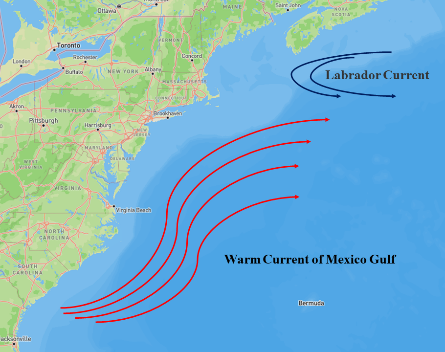
\includegraphics[width=0.30\textwidth]{test_22.png}}			  % 子图1的图片宽度 不能空行
    \subfigure[Large vs. Small Companies]{				% 图片2
    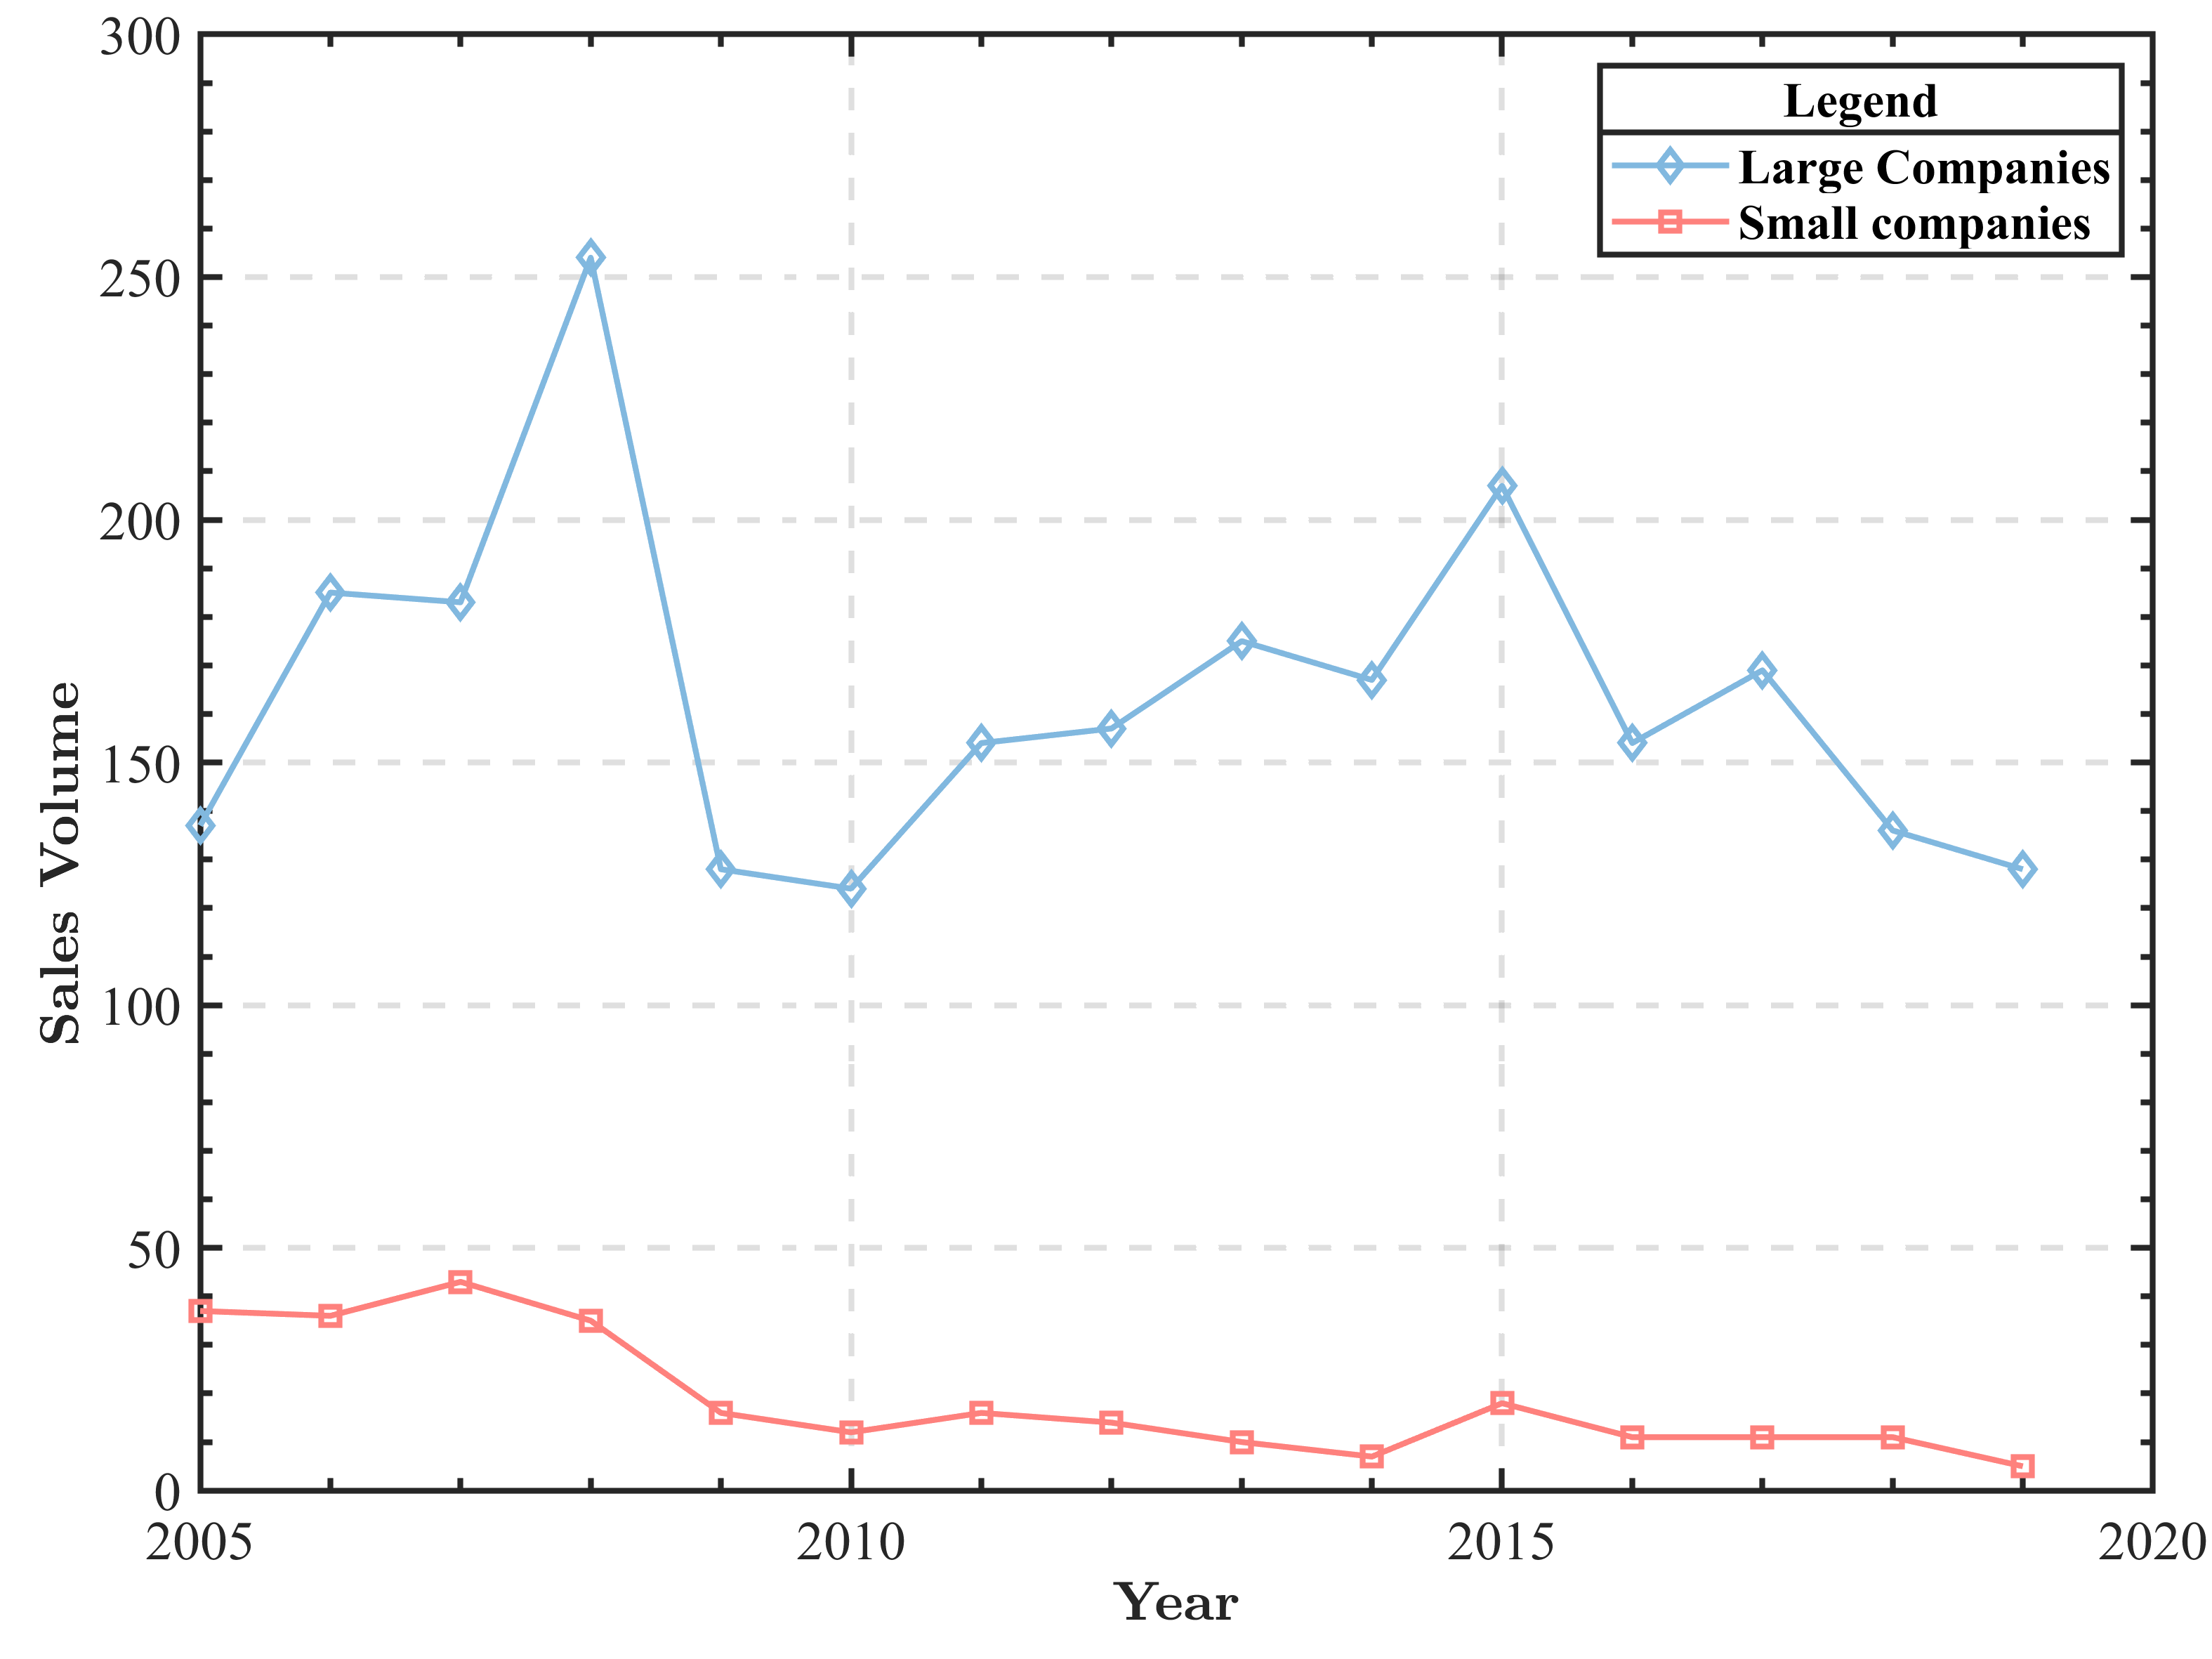
\includegraphics[width=0.315\textwidth]{test_23.png}} 
    \subfigure[Sales Price Stability]{				% 图片2
    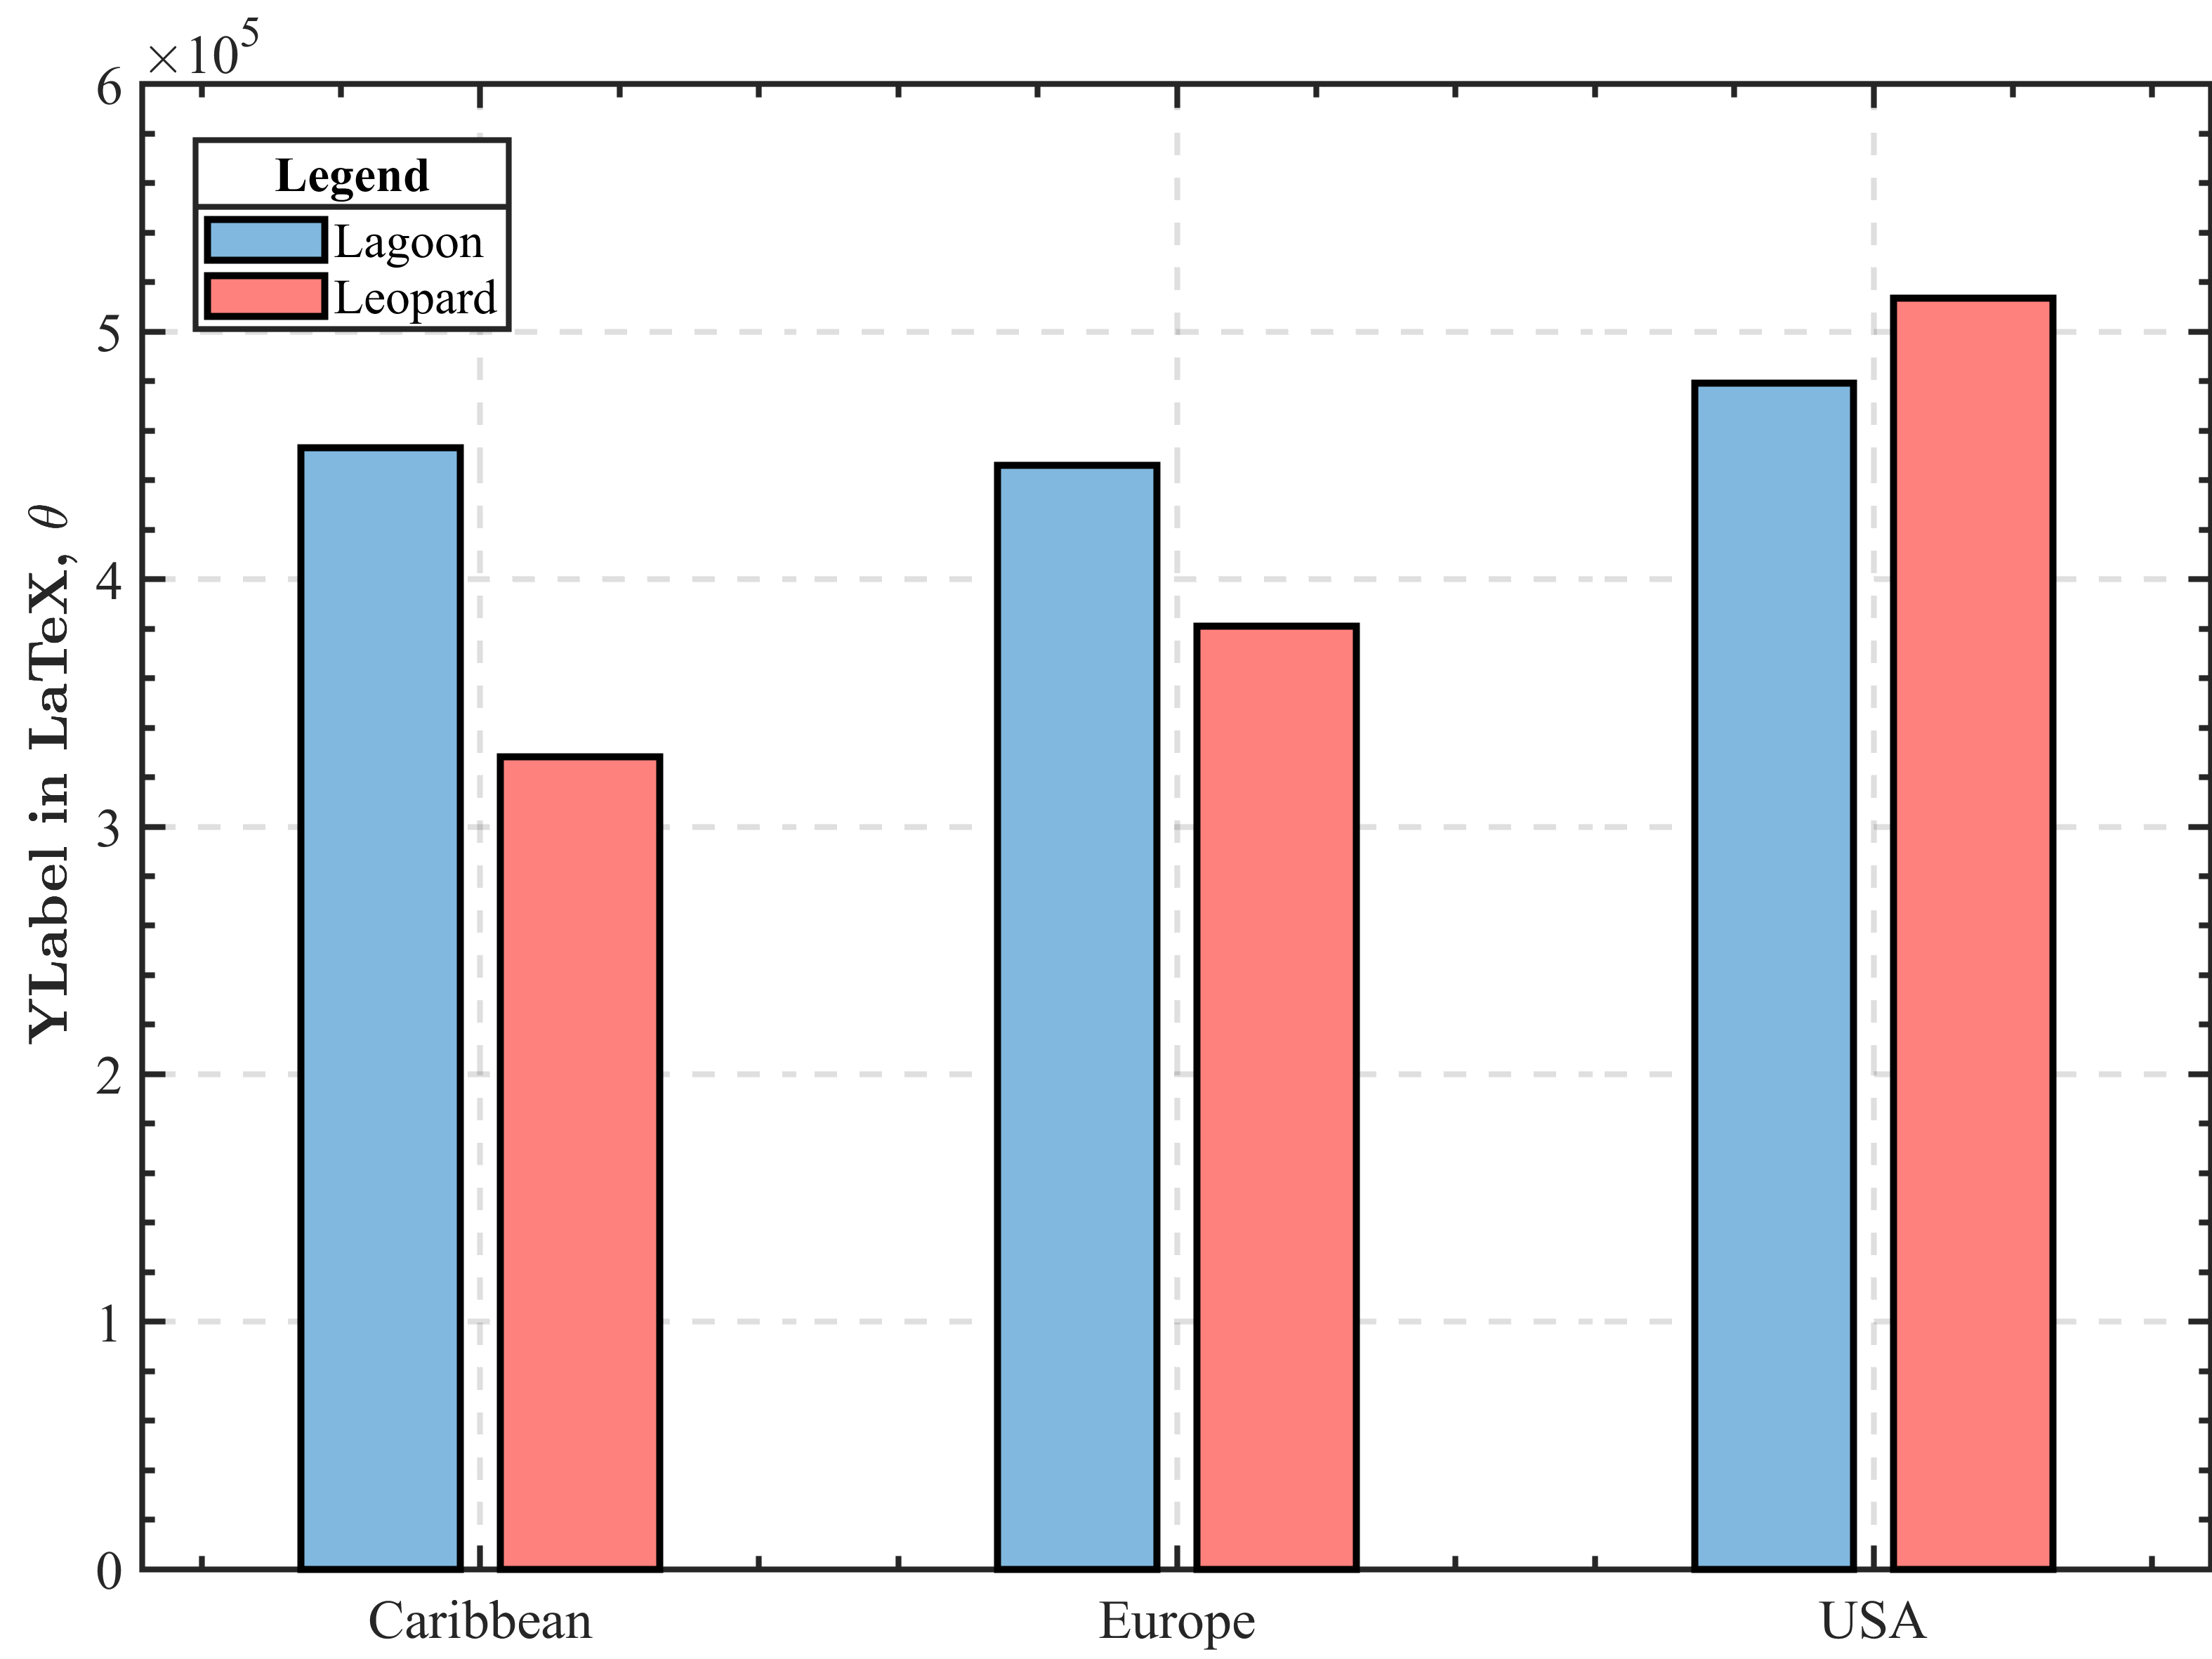
\includegraphics[width=0.315\textwidth]{test_24.png}} 
	\caption{RF, BP, and CNN Predicted Results Compared} % 图片标题 
    \vspace{-0.5cm}
\end{figure}

\subsection{Interesting Conclusions}
\begin{itemize}
    \setlength{\parsep}{0ex} %段落间距
    \setlength{\topsep}{2ex} %列表到上下文的垂直距离
    \setlength{\itemsep}{1ex} %条目间距
    \item We performed a year-by-year statistical comparison of used sailboats of monohull and double hulls. We found that the sales of monohulls are decreasing year by year while the number of catamarans is increasing year by year. This may be related to the increasing level of economic development and quality of recreation in different places.
    \item To explore the market for sailboats, we define sailboats that sell in each year and have an average selling price greater than \$500,000 as high-end market sailboats. Similarly, those with an average selling price of less than \$200,000 are called low end market sailboats.
    \item Our analysis of the annual sales of sailboats shows that some of them (e.g. Solona) alternate between sales and non-sales effects. We speculate that they may run an alternating sales-manufacturing operating model.
\end{itemize}

\begin{figure}[H] %[H]让图片在文章中的位置就是这段代码的位置
	\centering
		\begin{minipage}[t]{0.3\linewidth} %并排排列图片使用\minipage{}环境,而子图排列使用\subfigure{}环境
			\centering
			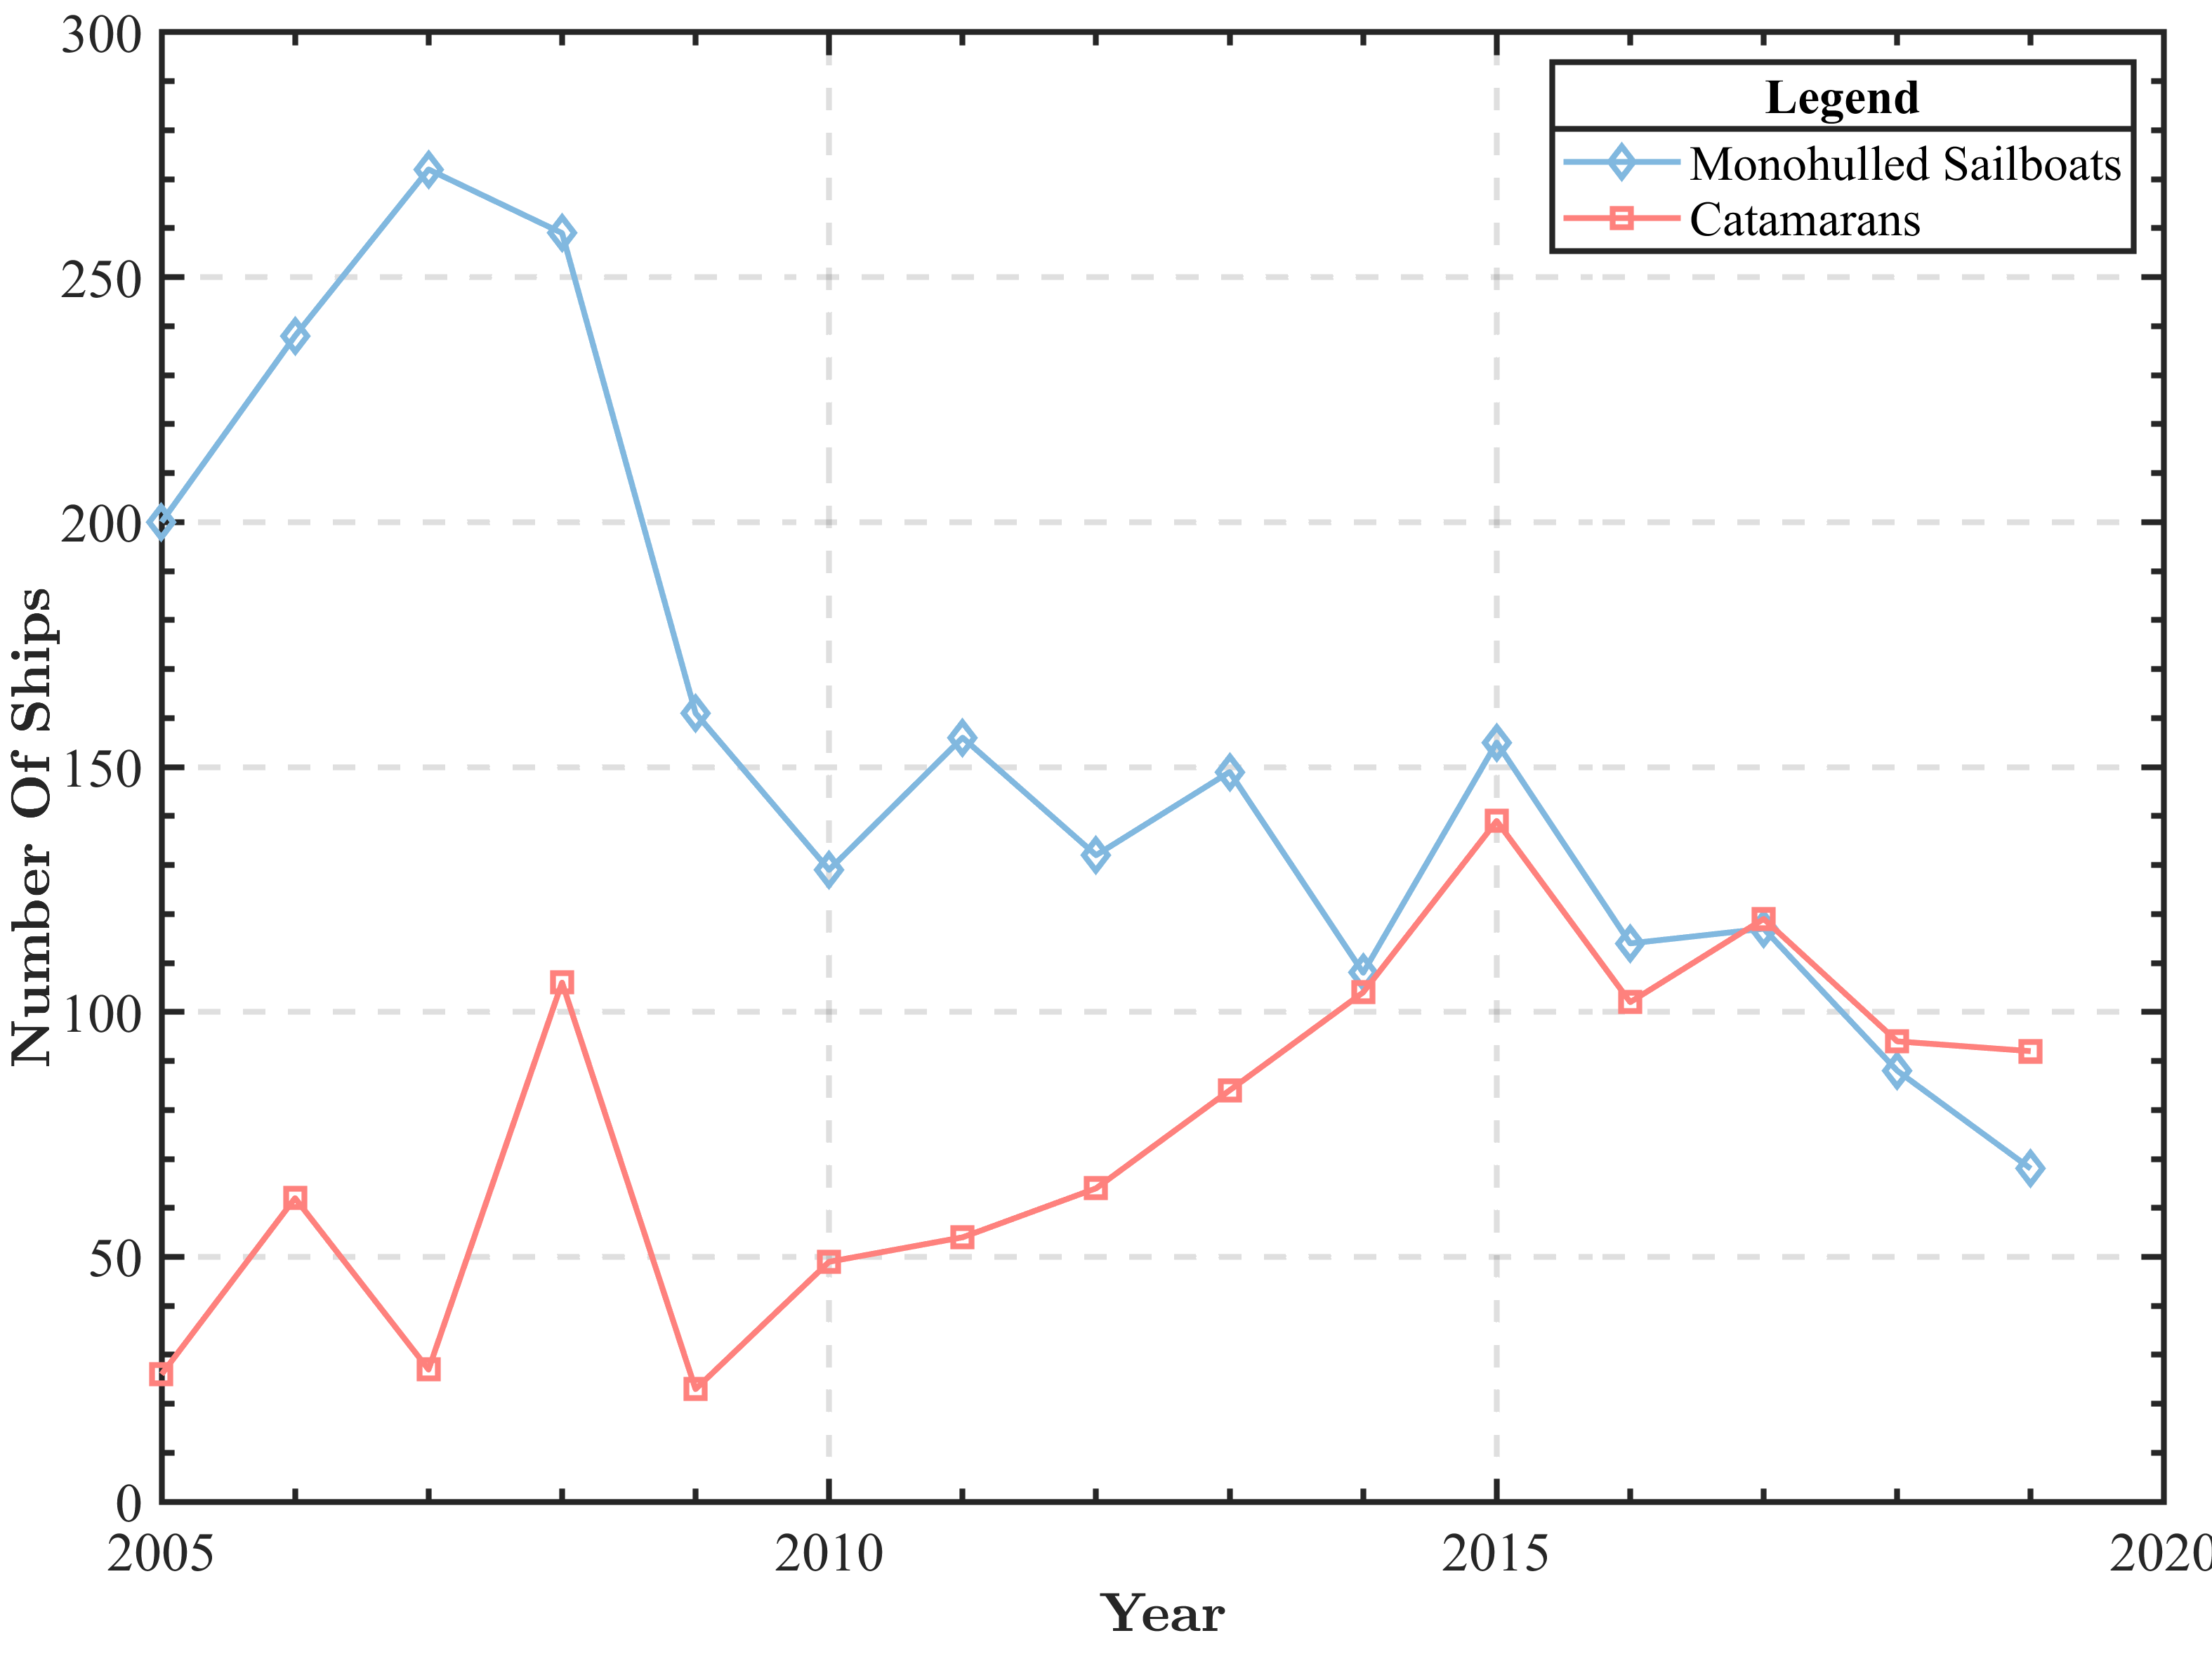
\includegraphics[width=0.9\linewidth]{test_25.png}
            \captionsetup{justification=centering} \caption{Monohull and Catamaran Trends}
		\end{minipage}%
		\begin{minipage}[t]{0.3\linewidth}
			\centering
			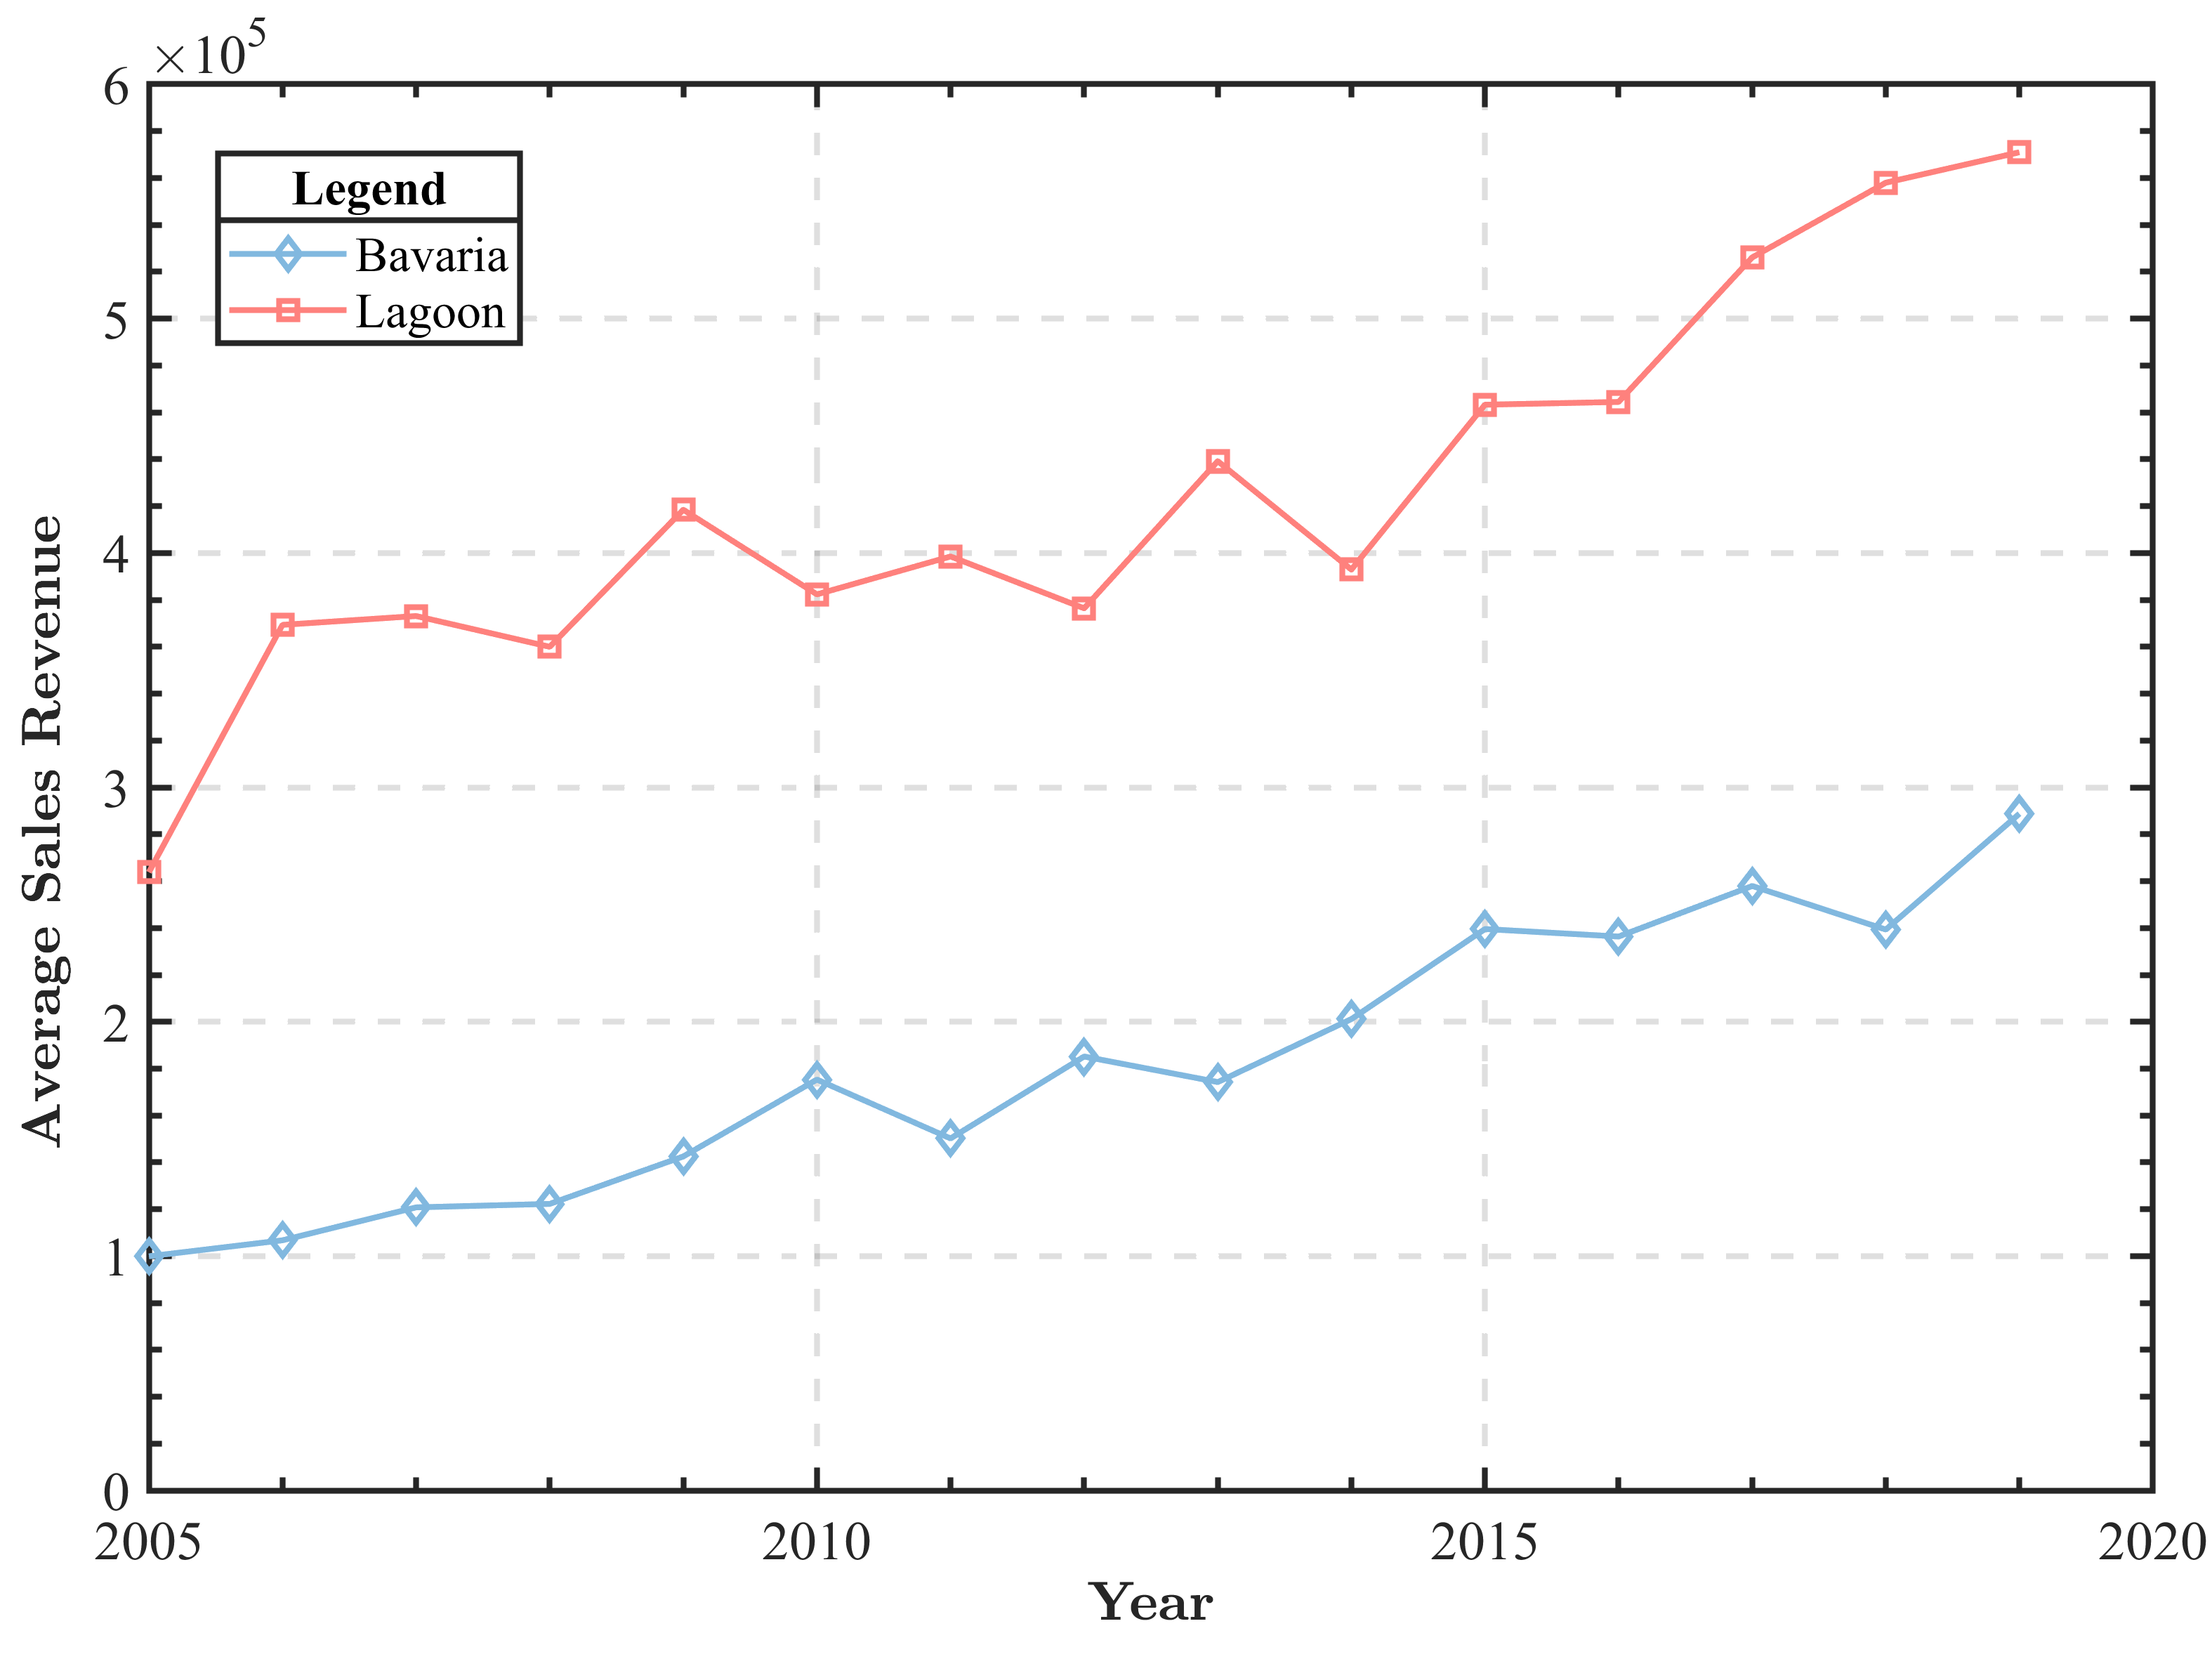
\includegraphics[width = 0.9\linewidth]{test_26.png}
			\captionsetup{justification=centering} \caption{A Comparison of the High and Low End of the Sailing Market}
		\end{minipage}%
        \begin{minipage}[t]{0.3\linewidth}
			\centering
			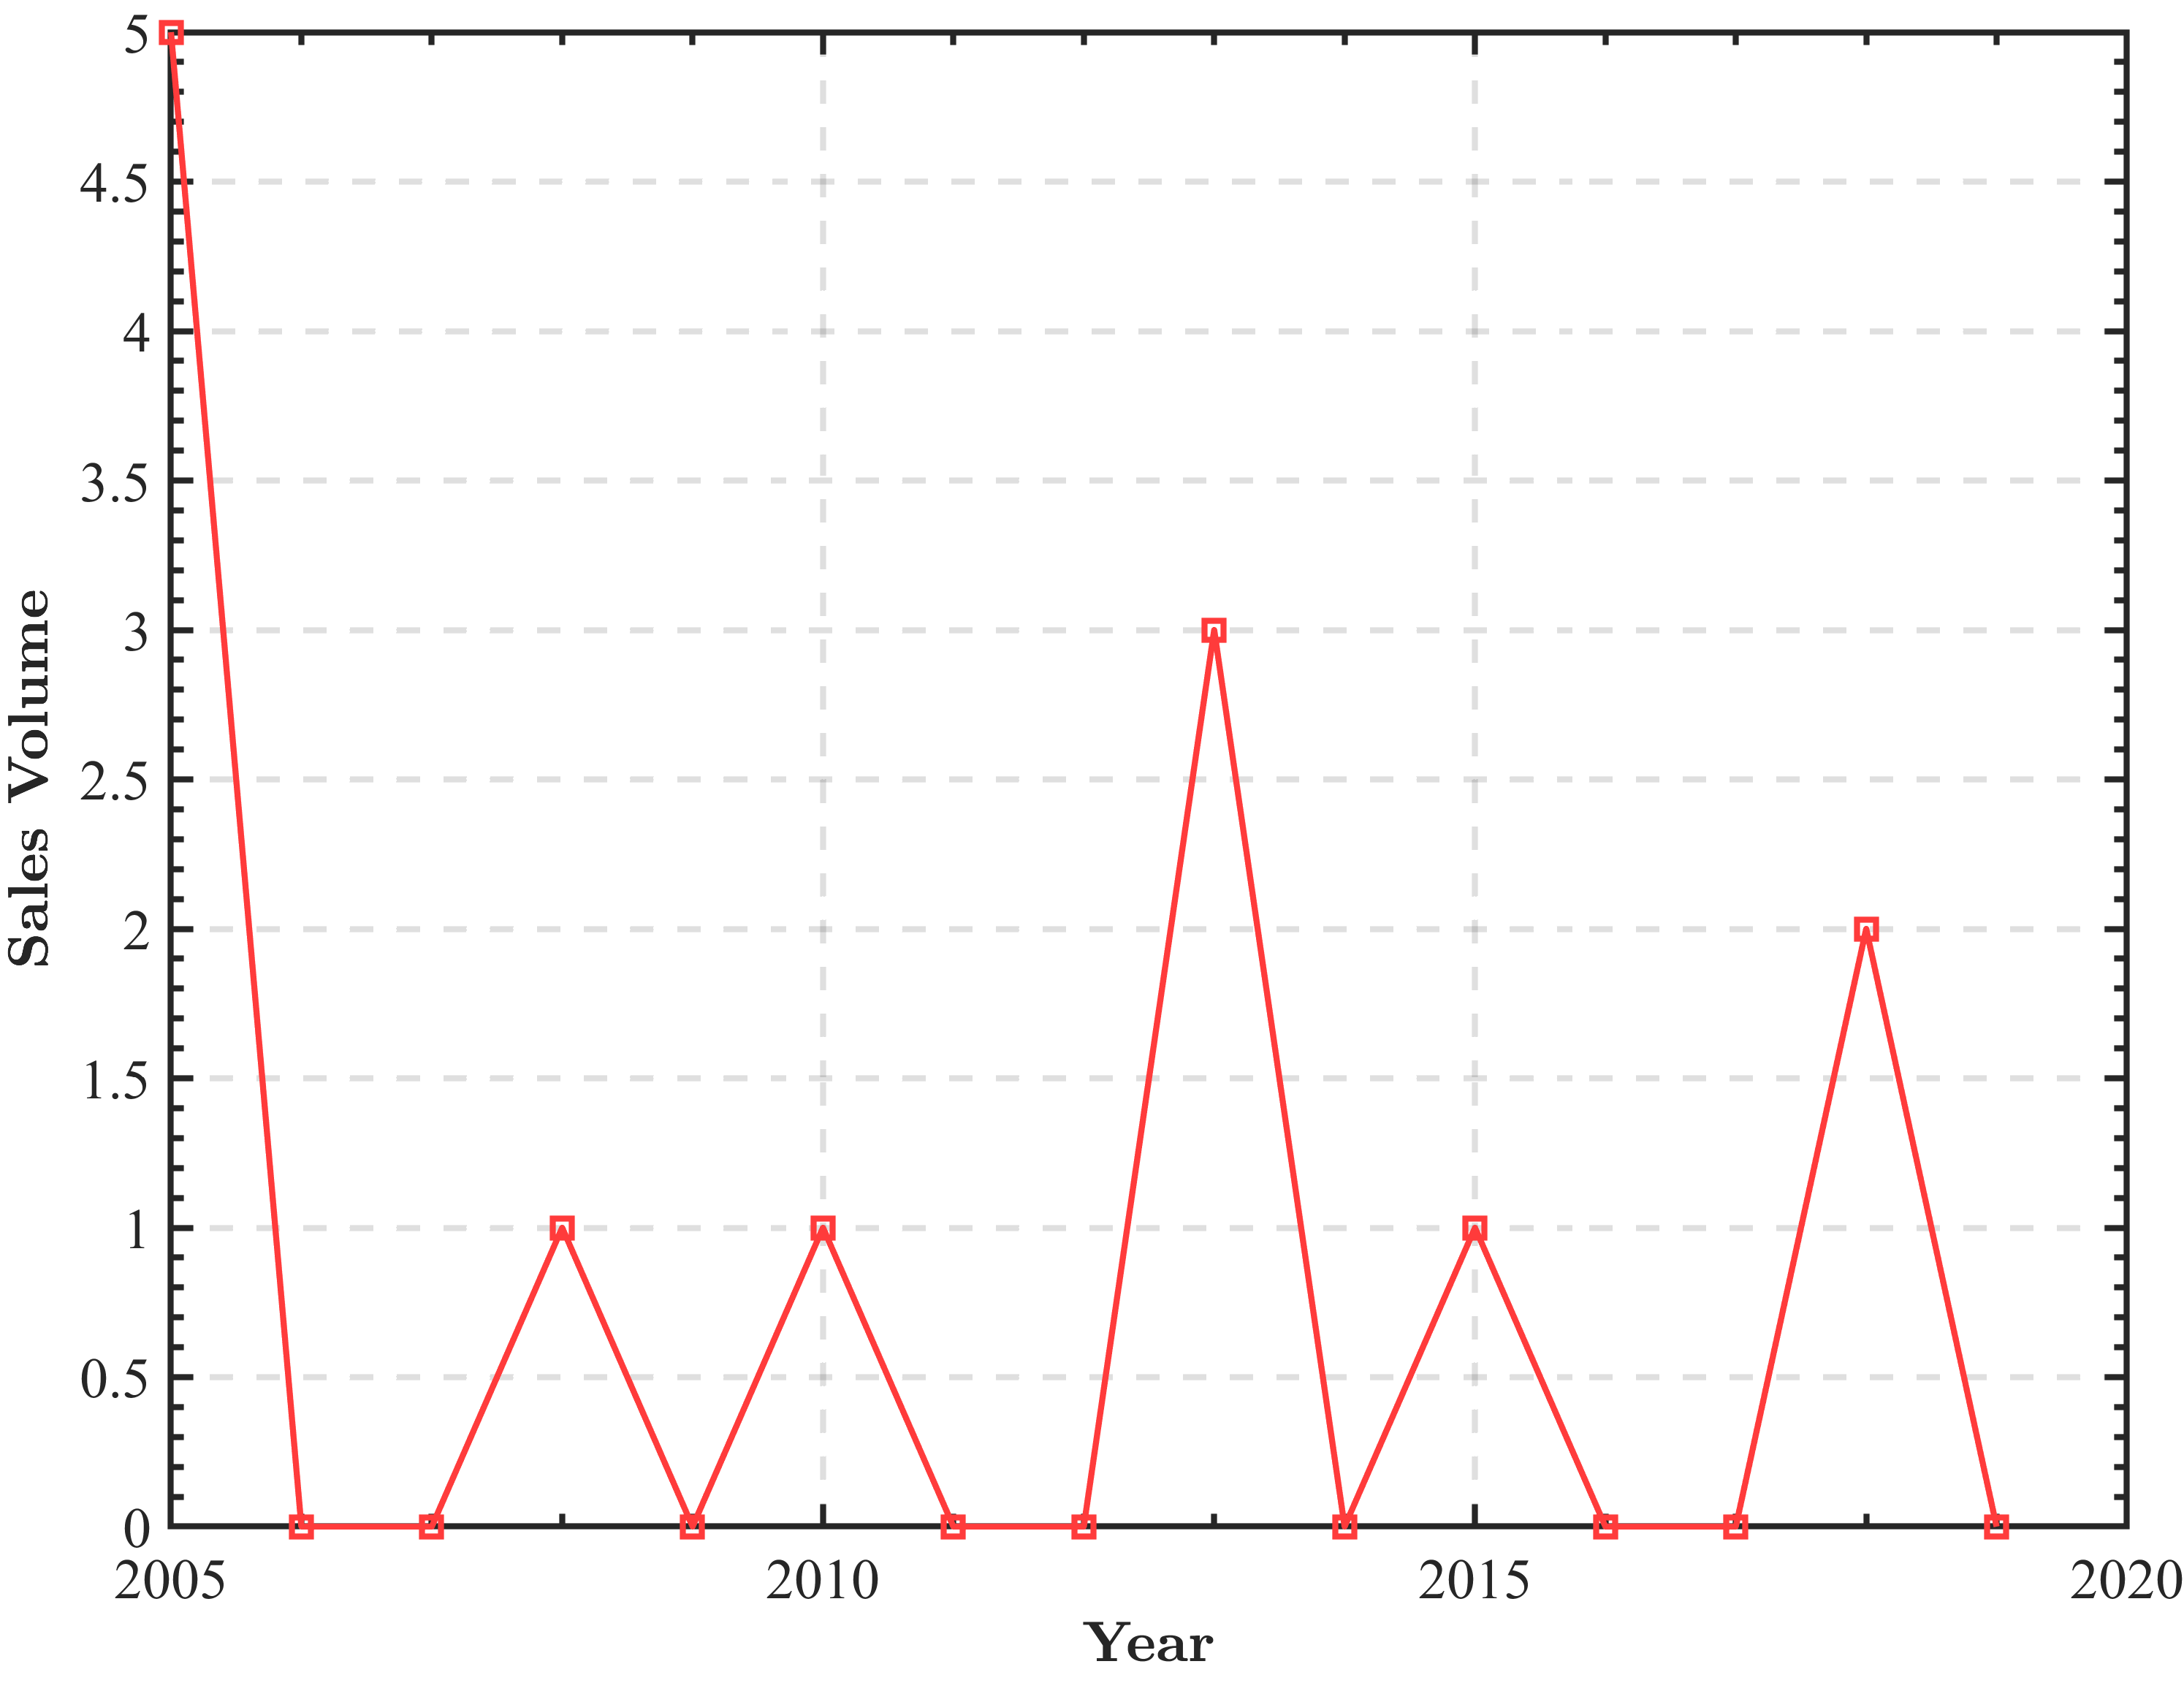
\includegraphics[width = 0.9\linewidth]{test_27.png}
			\captionsetup{justification=centering} \caption{ Solona Sales}
		\end{minipage}%
    \vspace{-0.5cm}
\end{figure}



\section{Sensitivity Analysis}
To verify the robustness of the model, we observe the changes by changing the input val-ues of the neural network.

\begin{itemize}
    \setlength{\parsep}{0ex} %段落间距
    \setlength{\topsep}{2ex} %列表到上下文的垂直距离
    \setlength{\itemsep}{1ex} %条目间距
    \item Sensitivity analysis of the fusion model\\
    We performed a sensitivity analysis of the fusion model in Problem 1 by changing the inputs to 0.95 to 1.05 of the original inputs for a total of 10 data sets and calcu-lating their mean error after removing the upper and lower quartiles. The results are shown in the following figure (a).
    \item Sensitivity Analysis of Data Forecasting in Hong Kong Region\\
    When forecasting the data for the Hong Kong region, we split the data into mono-hull and catamaran datasets. Change the input values to 0.95 to 1.05 of the original input values and observe the output as shown in figure (b) and figure (c) below.
\end{itemize}

\begin{figure}[H]
    \centering    
    \subfigure[Fusion Model]{				% 图片1([]内为子图标题)						
    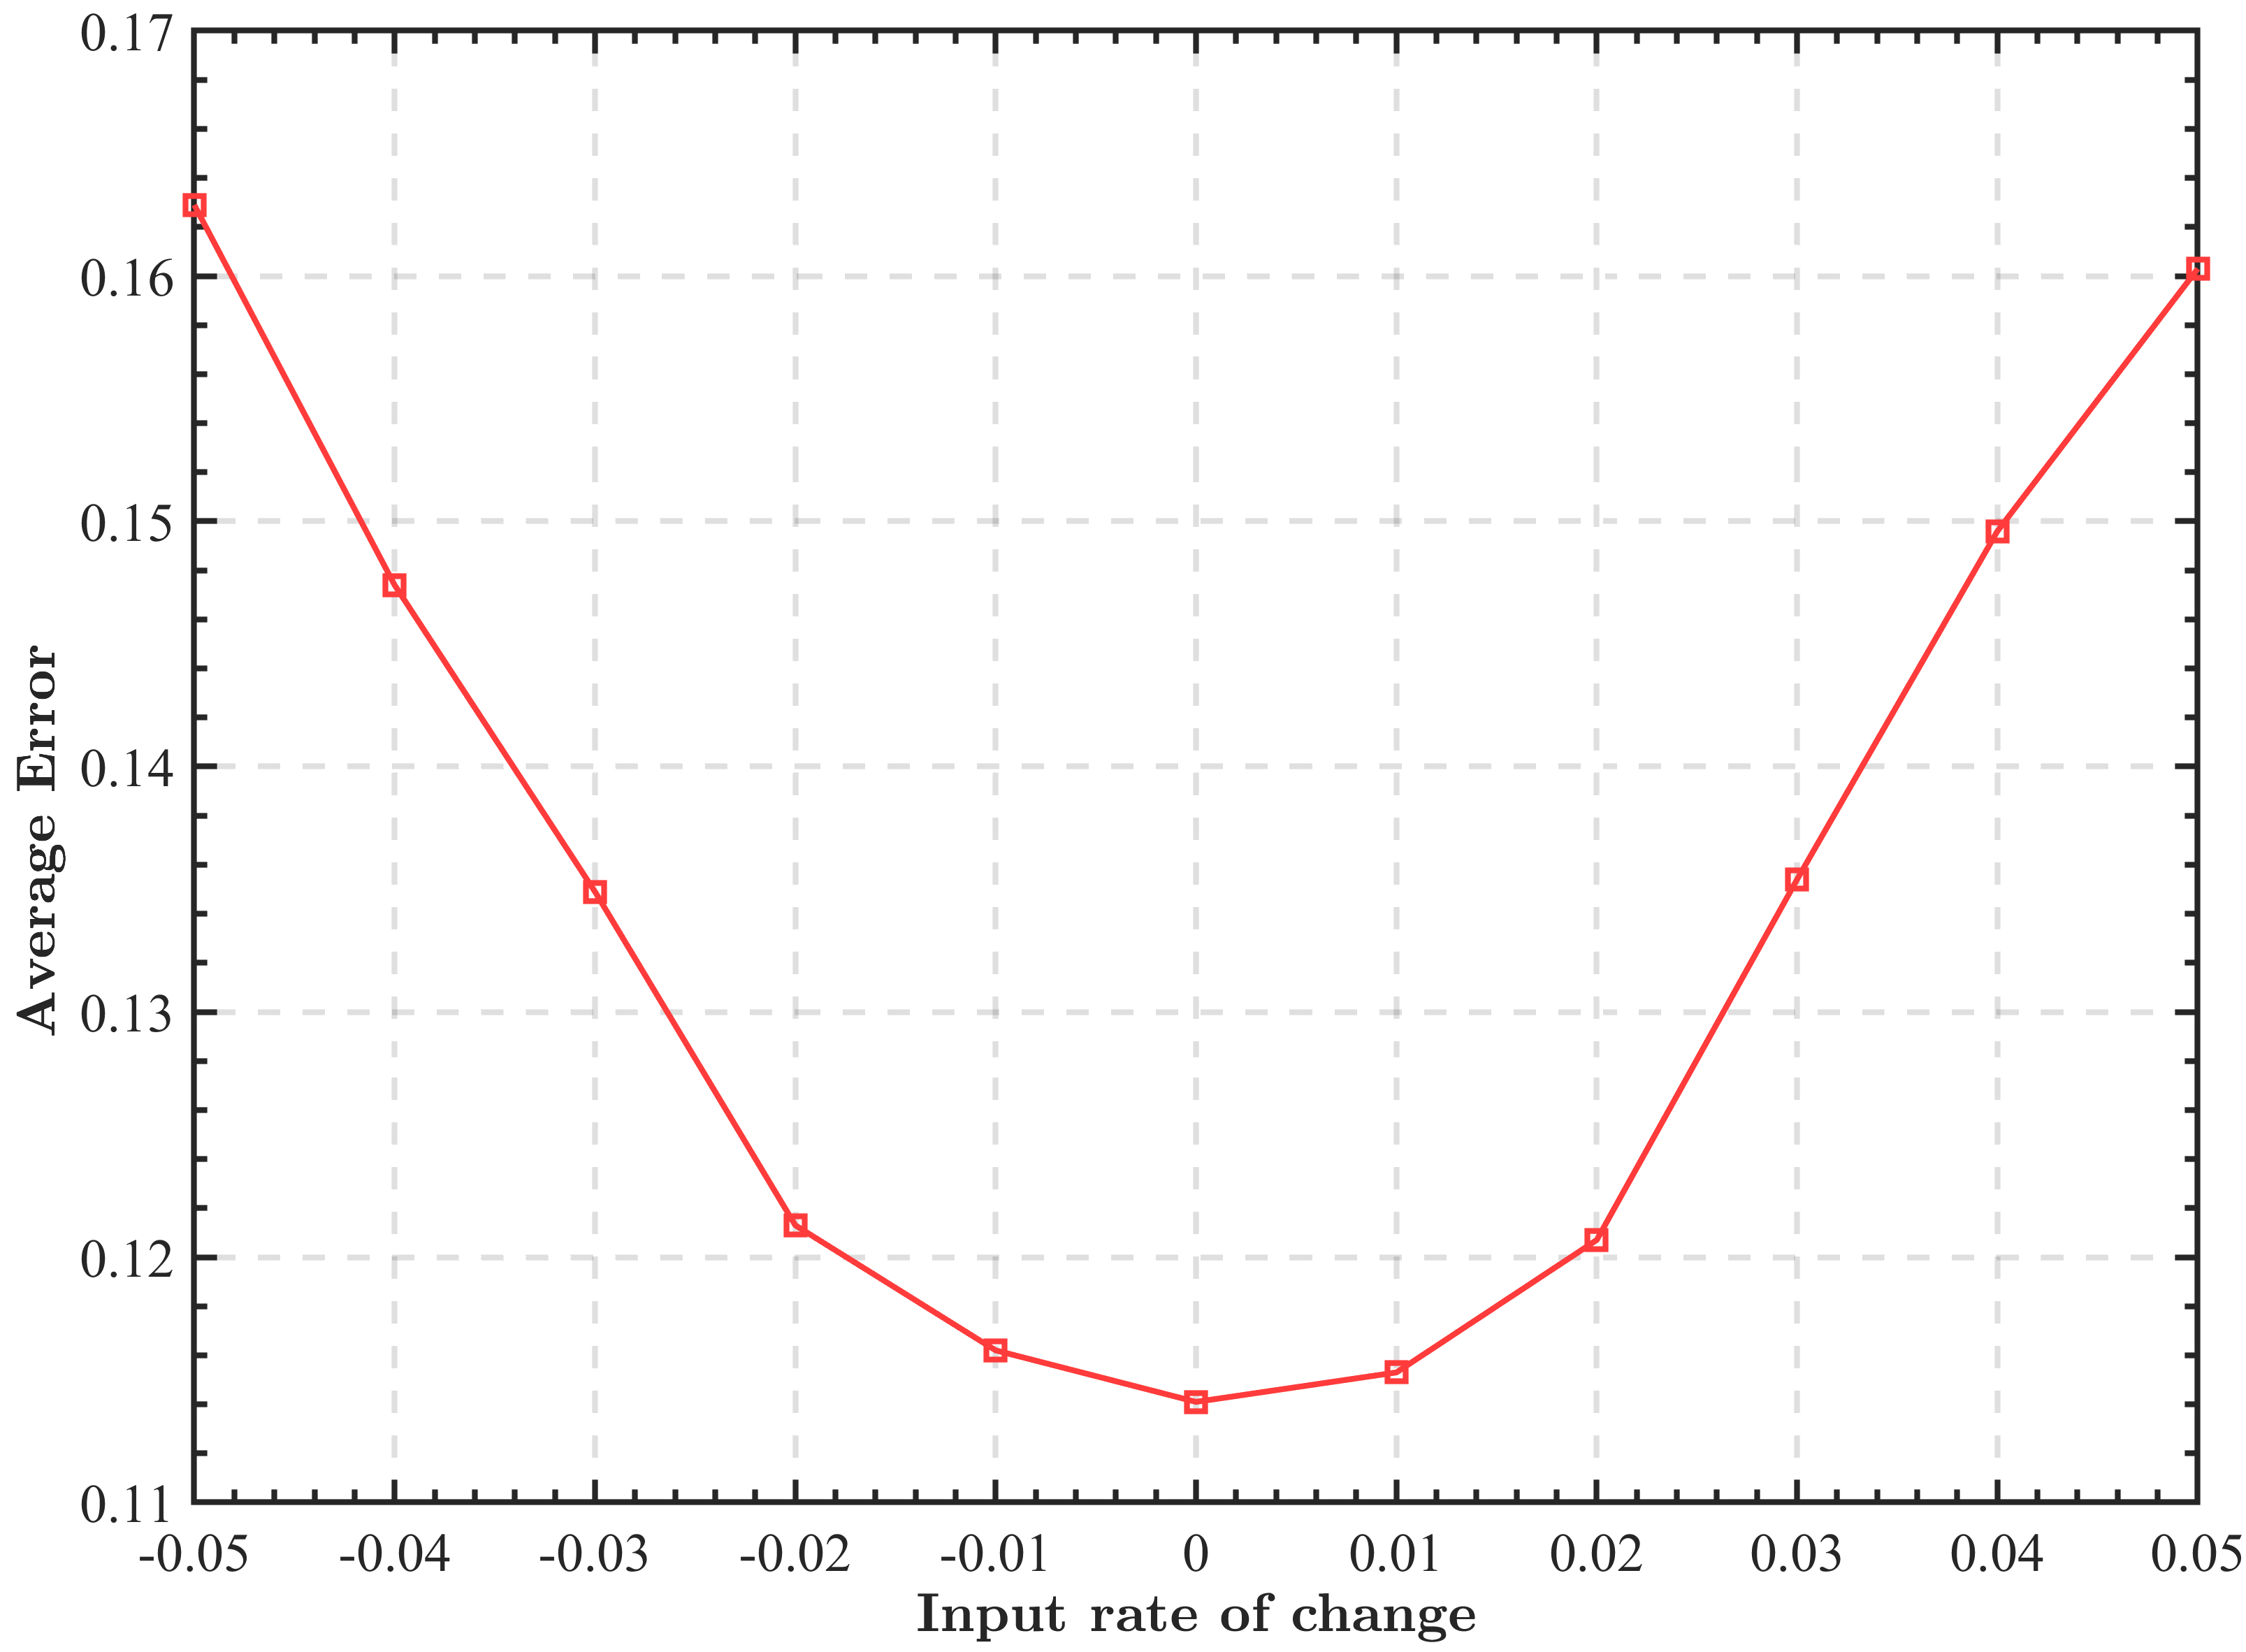
\includegraphics[width=0.31\textwidth]{test_28.png}}			  % 子图1的图片宽度 不能空行
    \subfigure[Monohull Forecast]{				% 图片2
    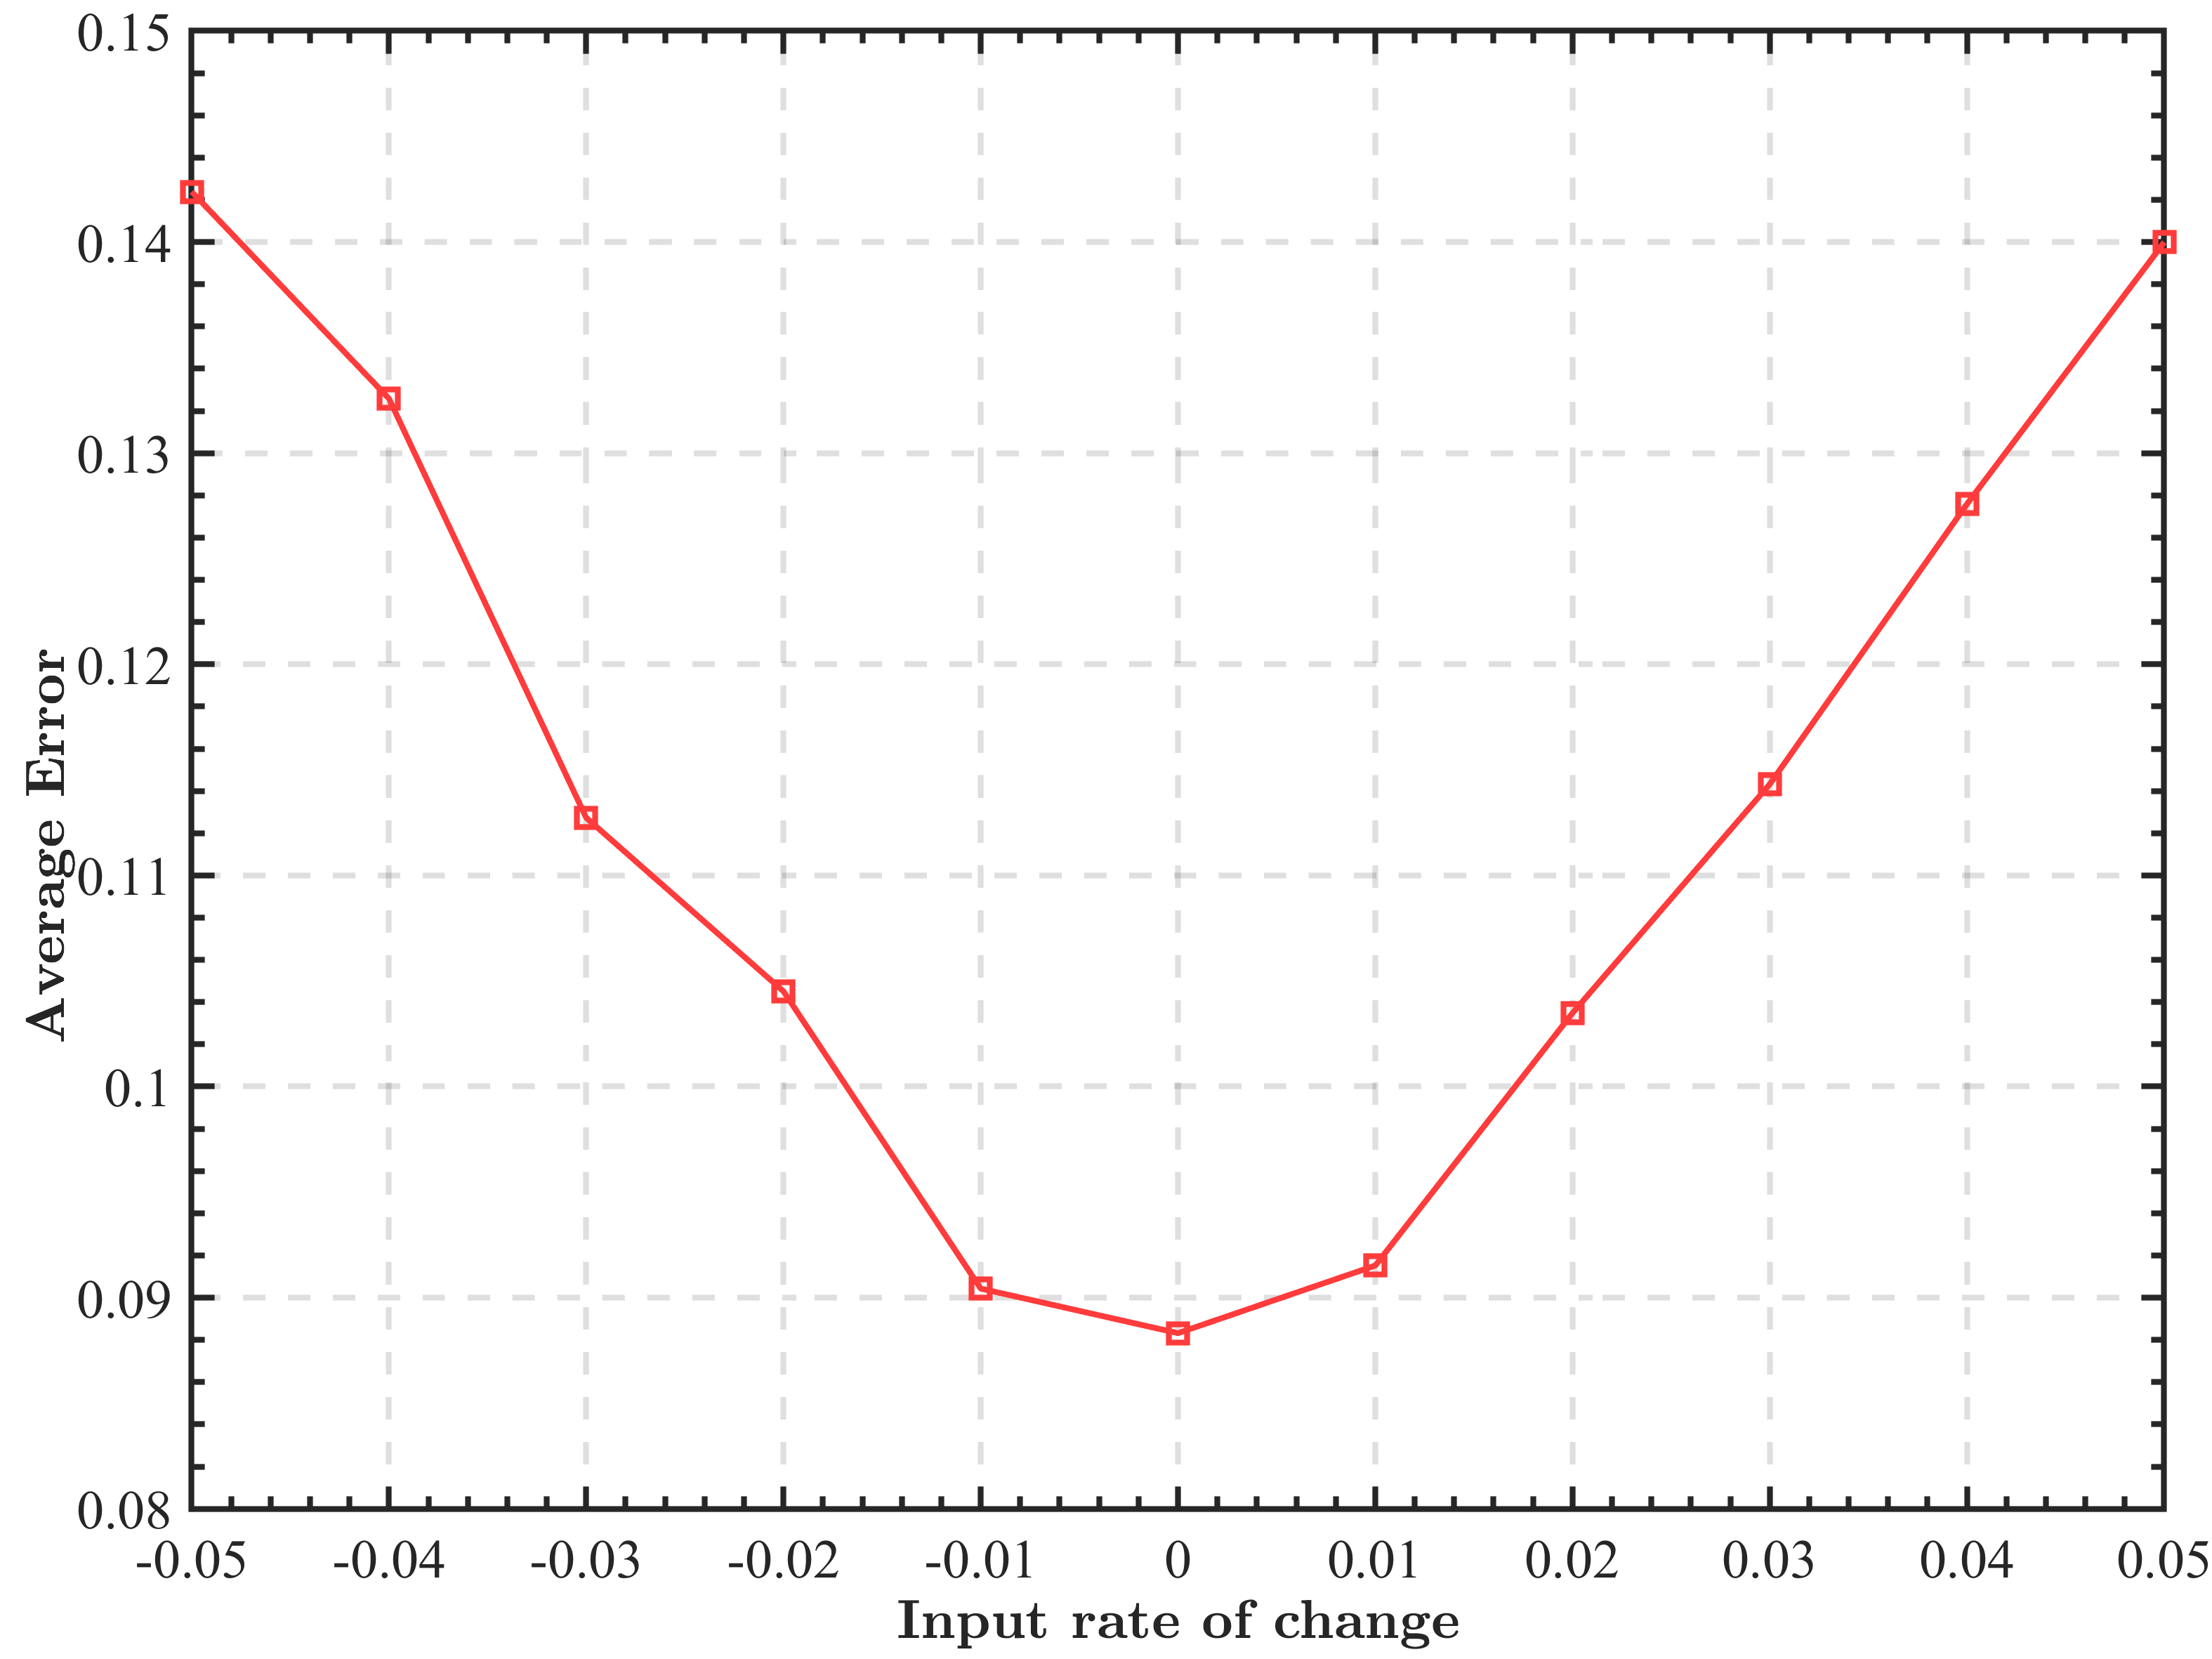
\includegraphics[width=0.31\textwidth]{test_29.png}} 
    \subfigure[Catamaran Forecast]{				% 图片2
    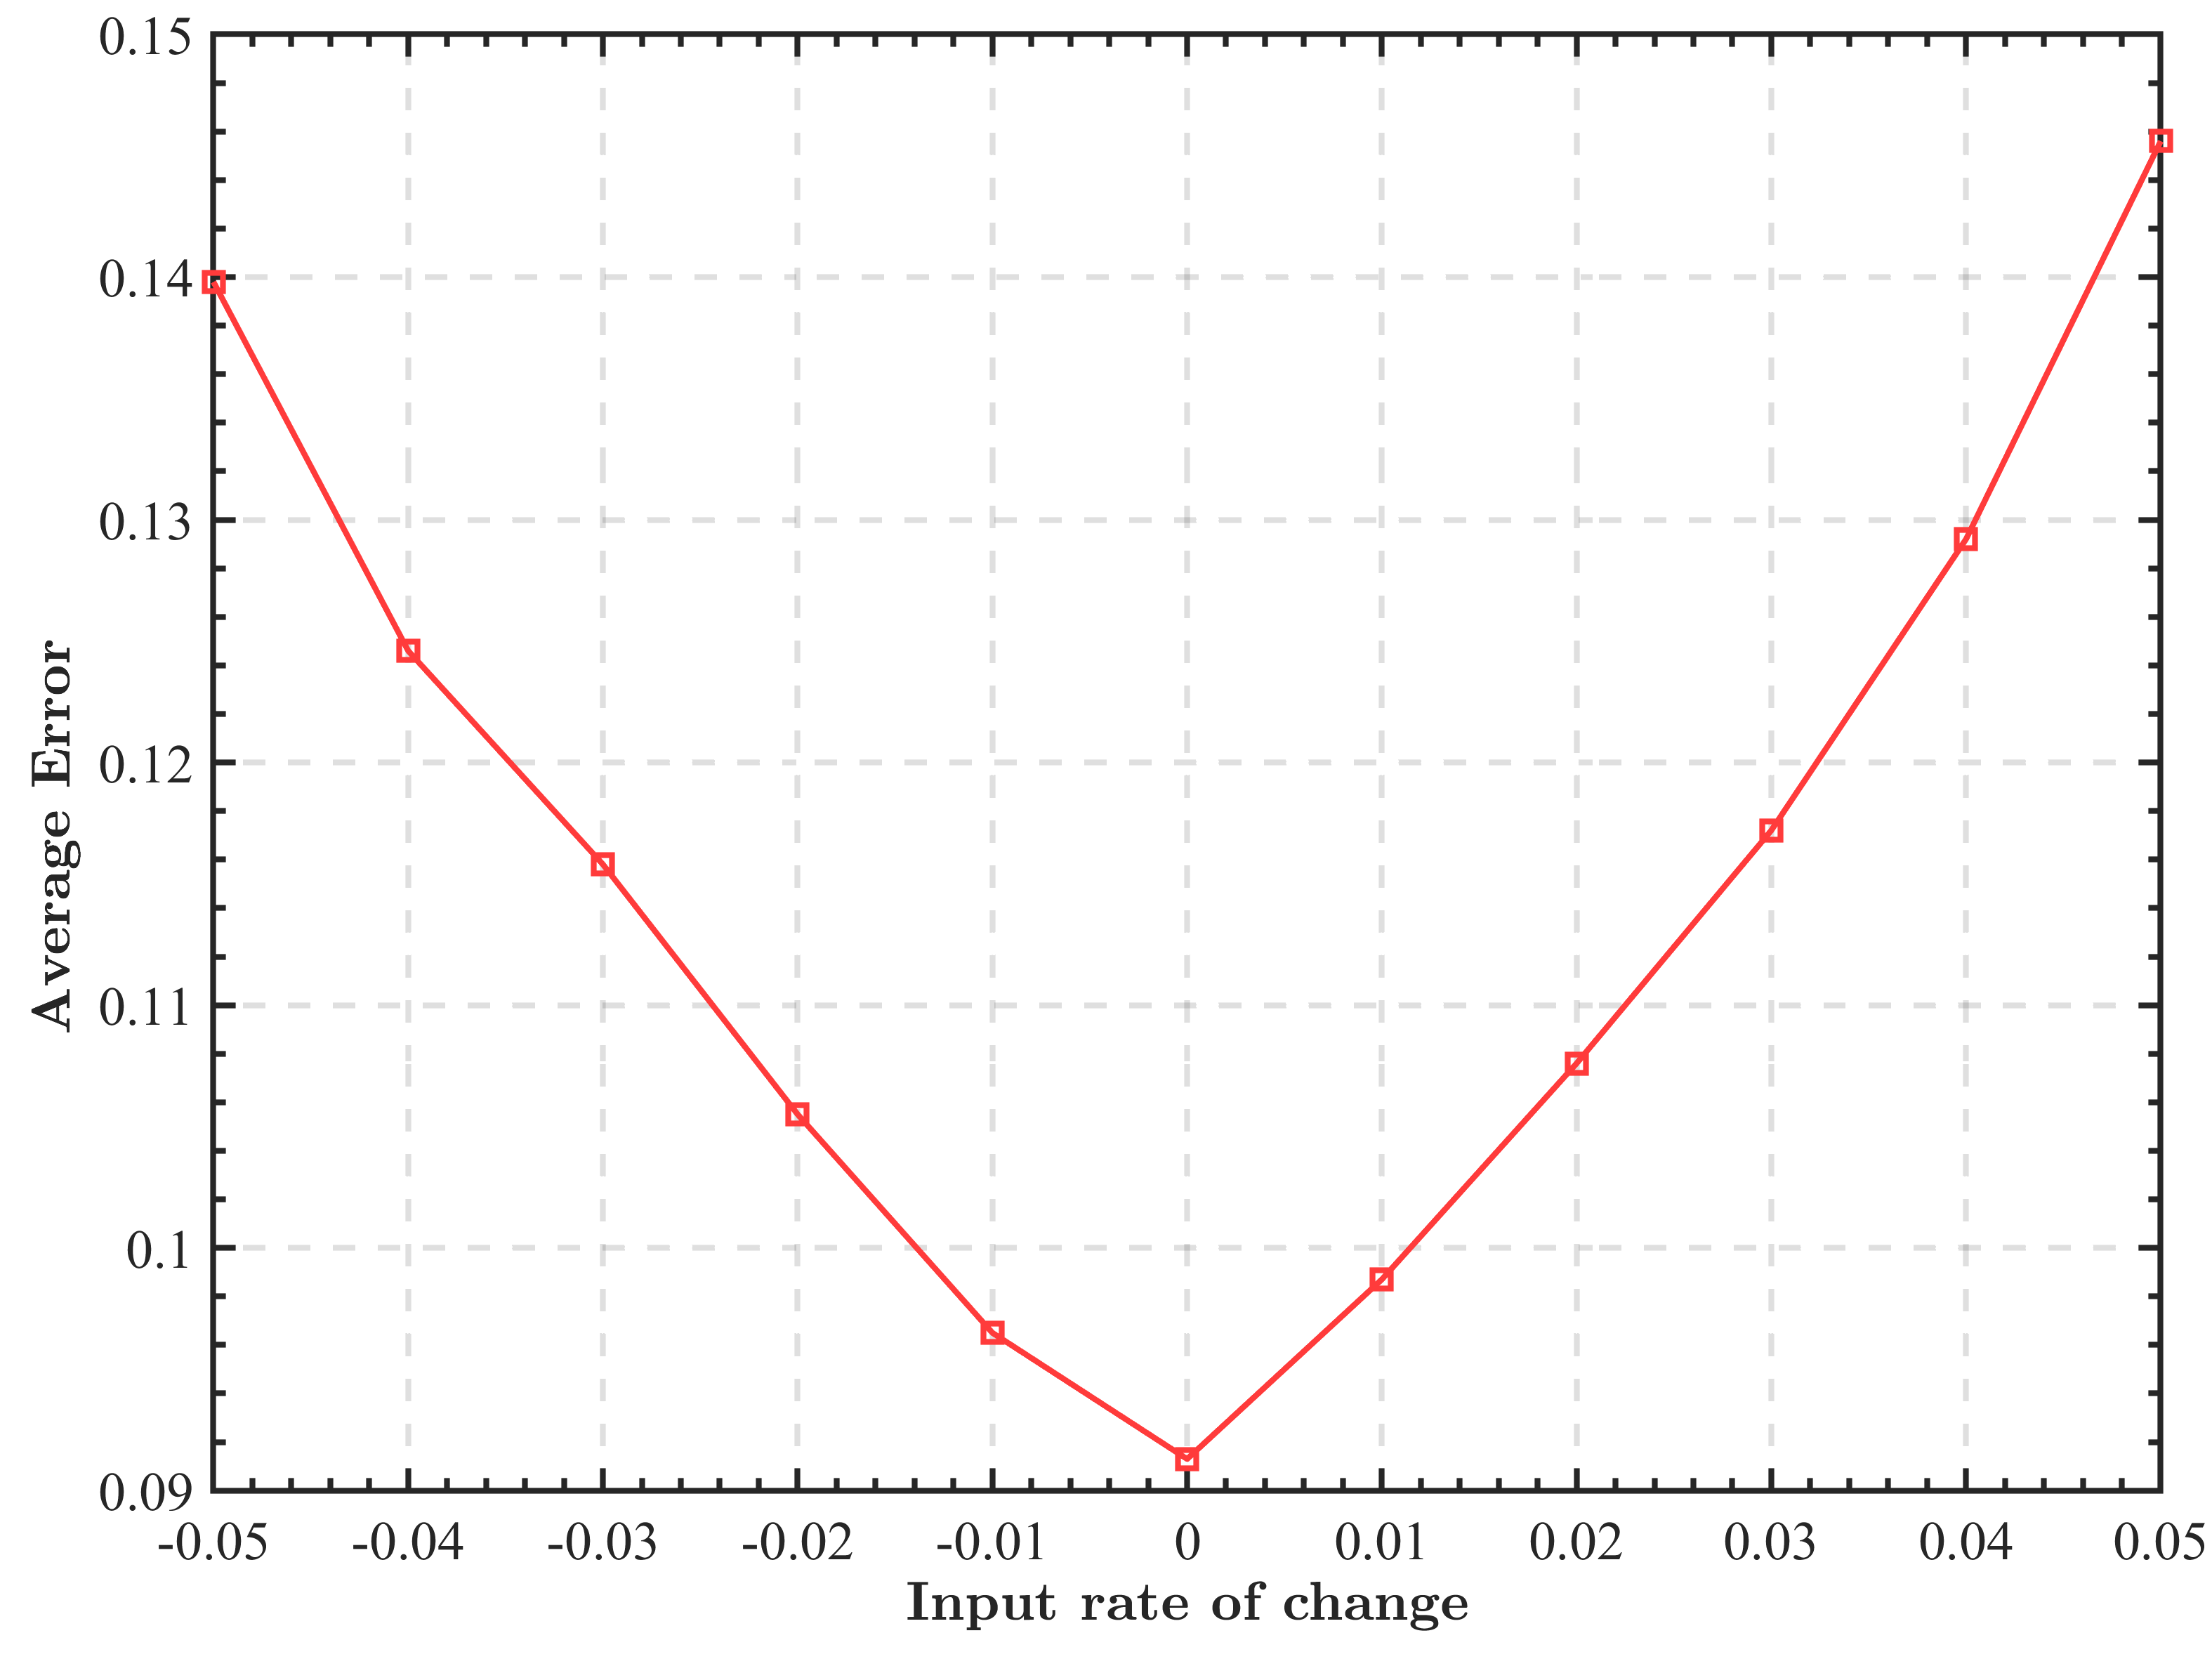
\includegraphics[width=0.31\textwidth]{test_30.png}} 
	\caption{Sensitivity Analysis of Each Neural Network} % 图片标题 
    \vspace{-0.5cm}
\end{figure}

As can be seen in the above figure (a), our fusion model exhibits better immunity to in-terference when the input values change. And from the two figures (b) and (c), we can see that the predicted data of the monohull is more resistant to interference. Although the pre-dicted data of catamaran is less resistant to interference but it does not vary much under the 5\% error band range, and the robustness of the model is better.

\section{Model Evaluation and Further Discussion}
\subsection{Strengths}
Our model offers the following strengths: 
\begin{itemize}
    \setlength{\parsep}{0ex} %段落间距
    \setlength{\topsep}{2ex} %列表到上下文的垂直距离
    \setlength{\itemsep}{1ex} %条目间距
    \item Our model has effectively achieved all the objectives, and it is based on the large data set of 12 parameter indicators of the sailboat, which has high reliability and stability;
    \item The visualization work is done very well by us, such as the research methodolog-ical framework of the article, the prediction effect of three intelligent algorithms and their fusion algorithms, the pie chart of the regional effect of variant sailboats, the chart of the prediction algorithm of sailboat prices in Hong Kong region, etc. Boring data may be able to reflect the law, but not as intuitive as so many images;
    \item We have more innovative and fusion methods, such as RF, the fusion of BP and CNN methods, the method of calculating regional effect indicators based on the change of sailboat ranking and the method of estimating the selling price of sail-boats in Hong Kong based on BP neural network.
\end{itemize}
\subsection{Weaknesses \texorpdfstring{$\&$} FFurther Discussion}
\begin{itemize}
    \setlength{\parsep}{0ex} %段落间距
    \setlength{\topsep}{2ex} %列表到上下文的垂直距离
    \setlength{\itemsep}{1ex} %条目间距
    \item The fusion of multiple models such as random forest may increase the time cost and complexity of the algorithm. In practice, the fused algorithms should be se-lected appropriately to balance the time cost and complexity cost;
    \item Since we did not find the actual selling price of sailboats in Hong Kong, the estimation results using BP neural network may be biased;
    \item The same predictions for used sailboats can be applied to products such as used cars and used houses. It provides guidance for the development of the used economy.
\end{itemize}

\section{Conclusion}
By analyzing the prices of used sailboats with their parameters, the regional effects of prices are also explored and eventually analyzed using Hong Kong, China as a validation for the region. Ultimately we obtained the following main conclusions.
\begin{itemize}
    \setlength{\parsep}{0ex} %段落间距
    \setlength{\topsep}{2ex} %列表到上下文的垂直距离
    \setlength{\itemsep}{1ex} %条目间距
    \item The relationship between regional indicators and the selling price of sailboats\\
    GDP per capita and average temperature are positively cor-related with sailing, in-dicating that people are more enthusiastic about water sports such as sailing when the economic level is higher or when the temperature is higher, which causes an increase in the selling price at that time. Precipitation and unemployment, on the other hand, reduce the sales of sailboats, which results in lower prices.
    \item Sailboats with significant price area effect\\
    The calculation of the change in the ranking of sailing boats allows us to obtain an indicator of the regional effect of sailing boats. After dividing according to this in-dicator, we found that the regional effect is not significant for the following types of boats: Hanse, Dufour, Leopard and Fountaine.
    \item The sales pattern of some sailboats\\
    From the known data, the sales of monohulls are decreasing while the sales of catamarans are increasing. At the same time there will be a clear regional effect for some sailing boats. When buying a sailboat, you should pay attention to the rela-tionship between the regional effect and the price.
\end{itemize}

In conclusion, these findings have greater implications for our study of pricing strate-gies for used sailboats and their regional effects. Also the study for the Hong Kong region can rapidly promote the economic development of the Hong Kong region.

%\begin{center}
%    \LaTeX\\
%    \Huge{\textxswup}\\
%    \normalsize{Word}
%\end{center}
